\section{Reproducible Numerical Validation}
The main experiments use finite directional laws, so expectations are evaluated directly as weighted sums without Monte Carlo error. Randomized linear-program objectives use independent streams from seed $20260919$; auxiliary checks use seed $20260918$. Information is in nats. Numerical angular searches are convergence checks, not certified global optimization.

\subsection{Nonzero Subspace Displacement and Cubic Regret}
Set $d=2$, $K=1$, and let $u_j=(\cos\alpha_j,\sin\alpha_j)$ occur with probability $p_j$, with
\begin{equation}
\begin{aligned}
(\alpha_1,\ldots,\alpha_4)&=(0,0.6,1.3,2.2),\\
(p_1,\ldots,p_4)&=(0.45,0.25,0.20,0.10).
\end{aligned}
\end{equation}
Angles are in radians. Write $P_\theta=v_\theta v_\theta^{\top}$ for the projector onto $v_\theta=(\cos\theta,\sin\theta)^{\top}$, and let $\theta_\gamma$ be a maximizing measurement angle. The leading eigenvector of $S_2$ has angle $\theta_0=\CoreAngle$, eigengap $\Delta=\CoreGap$, and contraction $A=\EE[x^3y]=\CoreA$, where $x=\cos(\alpha-\theta_0)$ and $y=\sin(\alpha-\theta_0)$. For Gaussian input, \eqref{eq:tilt} predicts $(\theta_\gamma-\theta_0)/\gamma\to-A/\Delta=\CoreTilt$. Consequently,
\begin{align}
\frac{\|P_\gamma-P_0\|_F}{\gamma}&\longrightarrow\CoreDistanceLimit,\\
\frac{\I_\mu^\star(\gamma)-\I_\mu(P_0;\gamma)}{\gamma^3}
&\longrightarrow\frac{A^2}{2\Delta}=\CoreRegretLimit.
\end{align}
We evaluate $21$ logarithmically spaced SNRs from $10^{-4}$ to $1$. Stationary angles are located by derivative sign changes on $8192$ angular intervals and refined by Brent's method; the best resulting value is selected. Doubling the angular resolution changes the selected information by less than $3\times10^{-17}$ nats. Regret is evaluated with a logarithmic ratio to reduce cancellation. On $10^{-4}\le\gamma\le10^{-2}$, fitted slopes are $\CoreDistanceSlope$ for distance and $\CoreRegretSlope$ for regret. Figure~\ref{fig:stability} compares these values with the analytic leading terms and finite-SNR bounds. The nonzero coefficient demonstrates that cubic regret cannot generally be replaced by a higher-order bound.
\begin{figure}[t]
\centering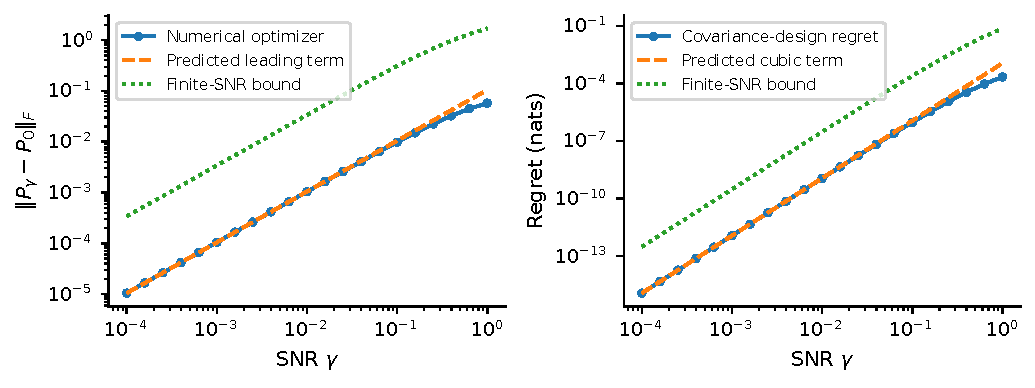
\includegraphics[width=0.95\textwidth]{figures/fig_optimizer_stability.pdf}
\caption{Gaussian four-direction example: numerical optimizer displacement (left) and covariance-design regret (right). Dashed curves use the derived leading coefficients; dotted curves are the explicit finite-SNR bounds.}
\label{fig:stability}
\end{figure}

To expose the geometry behind this displacement, embed the same four
directions as $u_j=(\cos\alpha_j,\sin\alpha_j,0)^\top\in\R^3$. Define
$b_0=(\cos\theta_0,\sin\theta_0,0)^\top$,
$b_1=(-\sin\theta_0,\cos\theta_0,0)^\top$, and $e_3=(0,0,1)^\top$.
The local unit-vector chart and its rank-one projector are
$v(t,s)=(b_0+t b_1+s e_3)/\sqrt{1+t^2+s^2}$ and
$P_{v(t,s)}=v(t,s)v(t,s)^\top$. At $\gamma=3$, denote by $P_3$ the
numerically selected information optimizer. Figure~\ref{fig:optimizer_chart_3d}
plots the information relative to the covariance projector $P_0$.
Any nonzero out-of-plane component $s$ reduces every coverage after
normalization, so an optimizer lies in the original plane; the visible
in-plane shift is the effect quantified by Corollary~\ref{cor:cubic_regret}.
\OptimizerChartFigure

\subsection{Equal Second Moments, Different Optimal Orientations}
Let $\mu_\phi$ assign equal mass to angles $\phi$ and $\phi+\pi/2$. For every $\phi$, $S_2=I_2/2$, whereas
\begin{equation}
M_2(P_\theta;\mu_\phi)=\frac38+\frac18\cos(4(\theta-\phi)).
\end{equation}
For Gaussian input and any positive SNR, the Jensen bound is attained exactly at $\theta=\phi+\pi/4$ modulo $\pi/2$, where both coverages equal $1/2$. Thus $\mu_0$ and $\mu_{\pi/6}$ have identical second moments and disjoint sets of optimal rank-one projectors. Figure~\ref{fig:orientation} shows their fourth-degree geometry and information at $\gamma=1$. This distinction is analytic; the plotted angular grid only displays it.
\begin{figure}[t]
\centering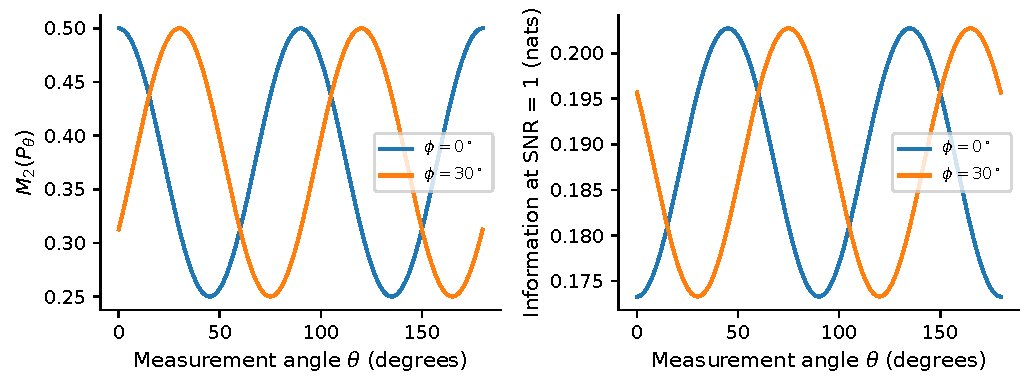
\includegraphics[width=0.95\textwidth]{figures/fig_orientation.pdf}
\caption{Two rotated directional laws with $S_2=I_2/2$. Minima of the fourth-degree coverage moment coincide with the exact information-maximizing orientations, which differ between the laws.}
\label{fig:orientation}
\end{figure}

\subsection{Compression of a Nonuniform Directional Law}
We take $41$ directions at $\alpha_j=\pi j/41$, $0\le j\le40$, with probabilities proportional to
\begin{equation}
\exp\{0.7\cos(2\alpha_j)+0.8\sin(4\alpha_j)+0.3\cos(6\alpha_j)\}.
\end{equation}
For $r\in\{1,2,3,4,6,8\}$, a linear program preserves the expectations of $1$, $\cos(2n\alpha)$, and $\sin(2n\alpha)$ for $1\le n\le r$. These functions span the even polynomial restrictions of degree at most $2r$ on the circle. A basic solution uses at most $2r+1=D_{2,r}$ directions. After least-squares refinement on the selected support, all weights remain positive; the maximum constraint residual is $\CoreMomentResidual$.

At SNRs $0.1$, $1$, and $10$, we compare original and surrogate information on $4096$ equally spaced measurement angles and transfer the numerically selected surrogate optimizer to the original law. The grid maximum is a sampled error, not the continuous supremum. At $r=4$ and $\gamma=1$, compression from $41$ to $9$ directions gives sampled information error $\CoreCompressionError$ and achieved transfer regret $\CoreCompressionRegret$ nats. The exact-matching theorem gives the respective reference bounds $1/810$ and $1/405$ nats. Figure~\ref{fig:compression} compares observed errors with these conservative guarantees. Different orders use independently chosen feasible supports, so monotonic observed error is not required.

Floating-point moment constraints are not asserted to hold exactly. The data also record a residual-aware Taylor bound from Theorem~\ref{thm:representation}(a)--(b); each coverage-moment error is at most the maximum Fourier constraint residual because the absolute Fourier coefficients of $\cos^{2n}(\theta-\alpha)$ sum to one. The plotted exact-matching bounds describe the ideal moment constraints. This deterministic compression experiment starts from a known finite law; the independent-sample guarantee is supplied separately by Corollary~\ref{cor:finite_sample}.
\begin{figure}[t]
\centering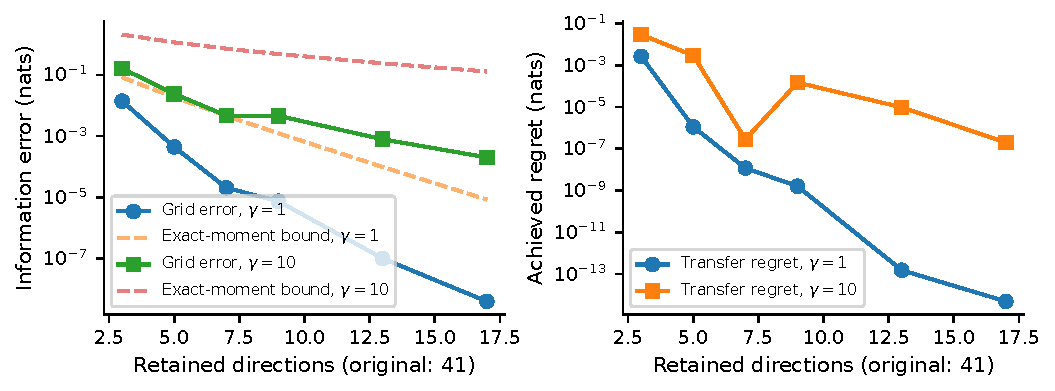
\includegraphics[width=0.95\textwidth]{figures/fig_surrogate.pdf}
\caption{Compression of a nonuniform 41-direction law. Left: sampled information errors and theoretical bounds for exact moment matching. Right: achieved transfer regret from numerical angular searches. Values below $10^{-16}$ are displayed at that floor.}
\label{fig:compression}
\end{figure}

\subsection{Finite-Sample Scaling Check}
For the same $41$-direction law and Gaussian SNR $\gamma=1$, we draw empirical
laws of sizes $N=100,400,1600$, and $6400$. Over $200$ independent repetitions,
we compute the maximum population-to-empirical information difference on the
same $4096$-angle grid. The median errors are, respectively,
$\CoreEmpiricalErrorA$, $\CoreEmpiricalErrorB$, $\CoreEmpiricalErrorC$, and
$\CoreEmpiricalErrorD$ nats. Their fitted log--log slope is
$\CoreEmpiricalSlope$, consistent with the $N^{-1/2}$ dependence in
Corollary~\ref{cor:finite_sample}. This is an empirical scaling check on a
finite angular grid, rather than a verification of the corollary's uniform
high-probability constant. The complete trial values are retained for
independent reanalysis.

\subsection{Rank-Two Design Transfer in Eight Dimensions}
To test compression beyond rank one, we fix $d=8$ and $K=2$. Define
\begin{equation}
\Sigma=\operatorname{diag}(8,5,3,2,1,1,1,1).
\end{equation}
Generate $600$ independent vectors $X_j\sim\mathcal N(0,\Sigma)$ and set $u_j=X_j/\|X_j\|$, with $u_{ji}$ denoting coordinate $i$ of direction $u_j$. The finite law assigns weights proportional to $\exp(0.6u_{j1}+0.4u_{j2}u_{j3})$. This realized finite law, not the underlying continuous Gaussian construction, is the target of compression. Reproduction uses seed $20260920$ with separate streams for directions, linear-program objectives, candidate projectors, and moment checks.

For matching orders $r=1,2$, positive linear programs preserve every homogeneous monomial of degree $2r$, together with total mass. Denote the resulting order-$r$ compressed law by $\nu_r$. Refined solutions retain $36$ and $330$ directions, respectively. At $r=3$, the support bound $D_{8,3}=1716$ exceeds the original $600$ directions, so we retain the original law as a reference rather than claim further compression. Checks on $128$ fresh projectors for each of ranks $2$ and $4$ give maximum coverage-moment residual $\RankResidual$. Thus the same surrogate weights are tested at more than one rank.

For each $\gamma\in\{1,10\}$, define a common finite candidate family $\mathcal Q_\gamma\subset\Pset$. It contains $512$ Haar projectors, the leading covariance projector, and $12$ projectors refined by projected-gradient ascent with orthonormalization. The refinements use four common starts for each of the original law and the two compressed laws. The resulting $\RankCandidates$ candidates are shared by all matching orders. Let $\widehat P_r$ maximize surrogate information over $\mathcal Q_\gamma$. Define the candidate-family information error $E_r^{\mathcal Q}$ and transfer regret $R_r^{\mathcal Q}$ by
\begin{align}
E_r^{\mathcal Q}&=\max_{P\in\mathcal Q_\gamma}|\I_\mu(P;\gamma)-\I_{\nu_r}(P;\gamma)|,\\
R_r^{\mathcal Q}&=\max_{P\in\mathcal Q_\gamma}\I_\mu(P;\gamma)-\I_\mu(\widehat P_r;\gamma).
\end{align}
These are the maximum error and transfer regret within the finite family. Exhaustive evaluation verifies $R_r^{\mathcal Q}\le2E_r^{\mathcal Q}$. The same comparison underlying Theorem~\ref{thm:representation}(a)--(b) applies to this restricted family, but these numerical values are not continuous-projector suprema or certified global-optimum regrets.

At $r=2$ and $\gamma=10$, the candidate information error is $\RankError$ nats and transfer regret is $\RankRegret$ nats. Figure~\ref{fig:rank_transfer} reports both quantities versus matching order. The third-order reference reproduces the original objective up to rounding because it uses the original law. This example directly tests measurement transfer for $K>1$ and also illustrates why an existence bound need not provide useful compression at every dimension and order.
\begin{figure}[t]
\centering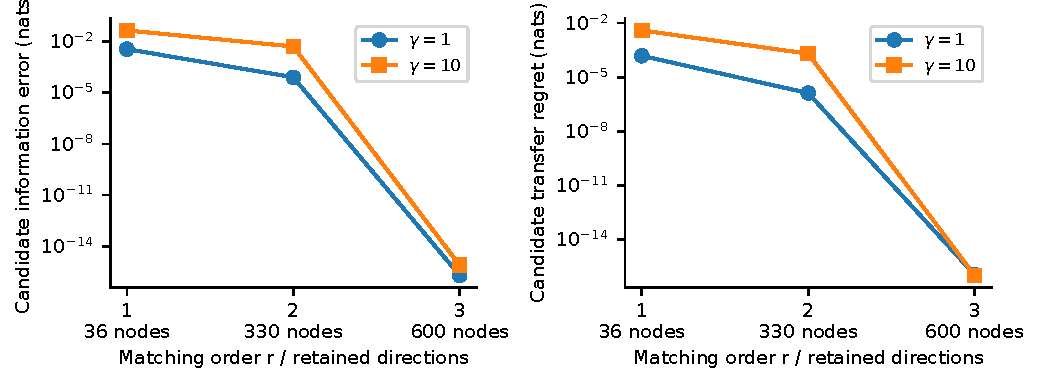
\includegraphics[width=0.95\textwidth]{figures/fig_rank_transfer.pdf}
\caption{Eight-dimensional rank-two design transfer over a common finite candidate family. Orders one and two use compressed laws; order three retains the original 600-direction law. Values below $10^{-16}$ are displayed at that floor. The curves do not certify optimization over all rank-two projectors.}
\label{fig:rank_transfer}
\end{figure}


\subsection{Auxiliary Reference Checks}
The accompanying auxiliary computation checks real and complex Haar coverage using $60000$ normalized Gaussian directions for each of $(d,K)=(3,1),(8,2),(8,4),(16,3)$. Maximum empirical Kolmogorov--Smirnov distances are $\KSReal$ and $\KSComplex$; these are sampling diagnostics. Exact finite-design curves from Proposition~\ref{prop:examples} have fitted low-SNR slopes $\SlopeAxes$ for axes/tetrahedron and $\SlopeIcosa$ for the icosahedral vertex witness. Across $1000$ random measuring directions, the latter ensemble's first two coverage moments match Haar to residual $\MomentError$.

The complex-channel normalization check is collected in Appendix~\ref{app:complex_check}.
